\documentclass[11pt]{article}

\usepackage[margin=1in]{geometry}
\usepackage{amsmath, amssymb}
\usepackage{graphicx}
\usepackage{booktabs}

\title{Root Finding in One and Several Dimensions}
\author{Ehsan Al Twal \\ Student Number: 89614622 \\ PHYS 410: Computational Physics}
\date{\today}

\begin{document}
\maketitle

%=======================================================================
\section{Introduction}
%=======================================================================

Bisection is guaranteed to converge but only linearly; Newton's method
converges quadratically but may diverge if started poorly. In Problem 1 I
combine the two into a hybrid scheme and use it to find all ten roots on
$[0,2]$ of
%
\begin{align}
f(x) = {}& 512x^{10} - 5120x^{9} + 21760x^{8} - 51200x^{7} + 72800x^{6} \nonumber \\
         & - 64064x^{5} + 34320x^{4} - 10560x^{3} + 1650x^{2} - 100x + 1 .
\label{eq:poly}
\end{align}
%
In Problem 2 I generalize Newton's method to $d$ dimensions and apply it to
%
\begin{equation}
x^2 + y^4 + z^6 = 2 , \qquad
\cos\!\left(x y z^2\right) = x + y + z , \qquad
y^2 + z^3 = (x + y - z)^2 ,
\label{eq:sys}
\end{equation}
%
near $\mathbf{x}^{(0)} = (-1.00,\, 0.75,\, 1.50)$.

%=======================================================================
\section{Review of theory}
%=======================================================================

\paragraph{Bisection.} If $f$ is continuous on $[a_0,b_0]$ with
$f(a_0) f(b_0) < 0$, the interval contains a root $x^\star$. Each step forms
the midpoint $x_n = \tfrac{1}{2}(a_n + b_n)$ and keeps the half with the sign
change, so
%
\begin{equation}
|x_n - x^\star| \le 2^{-(n+1)}(b_0 - a_0) ,
\label{eq:biserr}
\end{equation}
%
a linear rate of $\log_{10} 2 \approx 0.30$ digits per step.

\paragraph{Newton's method.} Linearizing $f$ about the current estimate $x_n$
and setting the result to zero gives the update
%
\begin{equation}
\delta_n = -\frac{f(x_n)}{f'(x_n)} , \qquad x_{n+1} = x_n + \delta_n .
\label{eq:newton}
\end{equation}
%
Each application of \eqref{eq:newton} is one step; the method repeats it until
$\delta_n$ is negligible. Near a simple root the error obeys
$e_{n+1} \approx \left[f''(x^\star)/2f'(x^\star)\right] e_n^2$, i.e.\ the
number of correct digits roughly doubles per step. In $d$ dimensions the step
becomes a linear system,
%
\begin{equation}
J(\mathbf{x}_n)\, \boldsymbol{\delta}_n = -\mathbf{f}(\mathbf{x}_n) ,
\qquad \mathbf{x}_{n+1} = \mathbf{x}_n + \boldsymbol{\delta}_n ,
\qquad J_{ij} = \frac{\partial f_i}{\partial x_j} ,
\label{eq:newtond}
\end{equation}
%
and convergence is again quadratic provided $J$ is nonsingular at the root.
There is no $d$-dimensional analogue of a bracket, so nothing plays the role
of bisection in Problem 2.

\paragraph{Exact roots of the test polynomial.} The leading coefficient
$512 = 2^9$ matches that of the Chebyshev polynomial $T_{10}$, and expanding
$T_{10}(u) = 512u^{10} - 1280u^8 + 1120u^6 - 400u^4 + 50u^2 - 1$ with
$u = x - 1$ reproduces \eqref{eq:poly} exactly, so $f(x) = T_{10}(x-1)$. Since
$T_{10}$ vanishes at $\cos[(2k-1)\pi/20]$,
%
\begin{equation}
x_k^\star = 1 + \cos\!\left(\frac{(2k-1)\pi}{20}\right) ,
\qquad k = 1, \dots, 10 ,
\label{eq:exact}
\end{equation}
%
which gives me an independent check on the computed roots.

%=======================================================================
\section{Numerical approach}
%=======================================================================

My function \texttt{hybrid} bisects until $b_n - a_n \le
\texttt{tol1}\cdot|x_n|$, then uses the final midpoint as the starting point
for Newton's method, repeating \eqref{eq:newton} until
$|\delta_n| \le \texttt{tol2}\cdot|x_{n+1}|$. My function \texttt{newtond}
repeats \eqref{eq:newtond}, solved with MATLAB's backslash operator, until
$\|\boldsymbol{\delta}_n\| \le \texttt{tol}\cdot\|\mathbf{x}_{n+1}\|$. Both
tests are relative, with a floor on the denominator in \texttt{hybrid} to cover
a root at the origin, and both routines have iteration caps.

I find the initial brackets by brute force: $[0,2]$ is sampled at $N = 10001$
points and each adjacent pair with $f(x_i) f(x_{i+1}) < 0$ is recorded. The
spacing $\Delta x = 2\times 10^{-4}$ is far below the smallest root separation
($\approx 9.7 \times 10^{-2}$), so no root is missed. The function, derivative,
residuals and Jacobian are all hard-coded analytically.

To reproduce the results, run \texttt{roots\_hybrid} (Problem 1:
Table~\ref{tab:roots}, Figures~\ref{fig:poly} and~\ref{fig:conv}) and
\texttt{test\_newtond} (Problem 2) from the MATLAB prompt in the HW1
directory. These scripts call \texttt{hybrid.m} and \texttt{newtond.m}
respectively.

%=======================================================================
\section{Results}
\label{sec:results}
%=======================================================================

\subsection{Problem 1}

With $\texttt{tol1} = 10^{-5}$ and $\texttt{tol2} = 10^{-12}$ the search found
exactly ten brackets and \texttt{hybrid} converged on each
(Table~\ref{tab:roots}). Every root agrees with \eqref{eq:exact} to a relative
accuracy between $10^{-15}$ and $6.2\times10^{-12}$; roots 1--7 meet the required $10^{-12}$, while roots 8--10 fall short by a factor of a few.

\begin{table}[htb]
\centering
\begin{tabular}{clll}
\toprule
$k$ & Computed root & Exact root, Eq.~\eqref{eq:exact} & $|f(x_k)|$ \\
\midrule
 1 & 0.012311659404862 & 0.012311659404862 & $1.110 \times 10^{-16}$ \\
 2 & 0.108993475811632 & 0.108993475811632 & $1.443 \times 10^{-15}$ \\
 3 & 0.292893218813453 & 0.292893218813453 & $1.421 \times 10^{-14}$ \\
 4 & 0.546009500260421 & 0.546009500260453 & $1.359 \times 10^{-13}$ \\
 5 & 0.843565534959918 & 0.843565534959769 & $1.117 \times 10^{-12}$ \\
 6 & 1.156434465039169 & 1.156434465040231 & $8.584 \times 10^{-12}$ \\
 7 & 1.453990499739204 & 1.453990499739547 & $4.599 \times 10^{-11}$ \\
 8 & 1.707106781179397 & 1.707106781186547 & $7.774 \times 10^{-12}$ \\
 9 & 1.891006524176727 & 1.891006524188368 & $3.657 \times 10^{-10}$ \\
10 & 1.987688340592448 & 1.987688340595138 & $7.740 \times 10^{-10}$ \\
\bottomrule
\end{tabular}
\caption{Roots of Eq.~\eqref{eq:poly} on $[0,2]$ from the hybrid algorithm,
with $\texttt{tol1} = 10^{-5}$ and $\texttt{tol2} = 10^{-12}$, compared against
the exact values \eqref{eq:exact} and shown with the residual at each computed
root.}
\label{tab:roots}
\end{table}

\begin{figure}[htb]
\centering
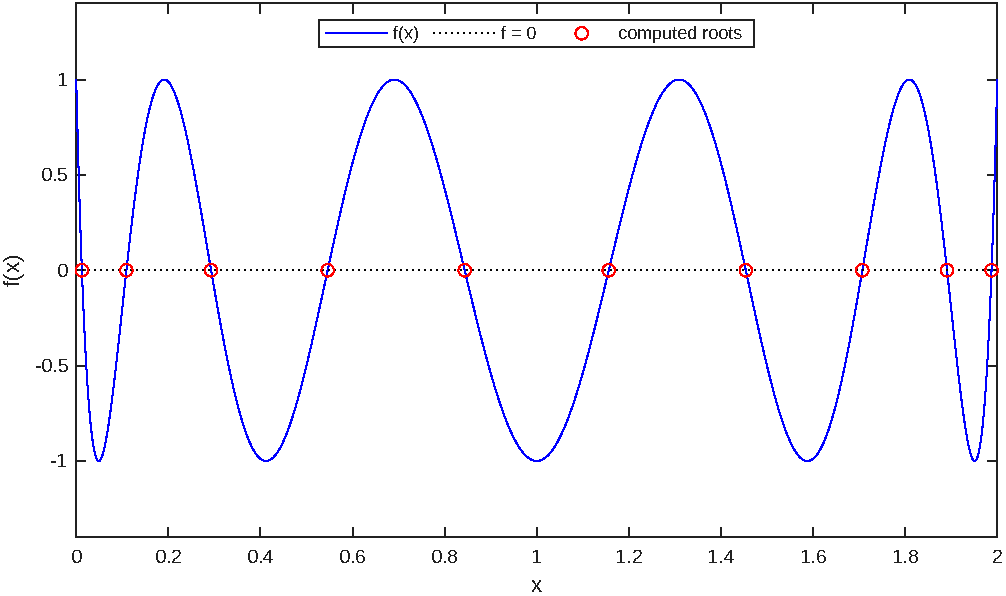
\includegraphics[width=0.78\textwidth]{fig1_polynomial.pdf}
\caption{The test polynomial and its ten computed roots. Eq.~\eqref{eq:poly}
over $[0,2]$, with the roots returned by \texttt{hybrid} marked as circles.
As $f(x) = T_{10}(x-1)$, the function oscillates between $\pm 1$ with its
zeros clustered towards the ends of the interval.}
\label{fig:poly}
\end{figure}

\begin{figure}[htb]
\centering
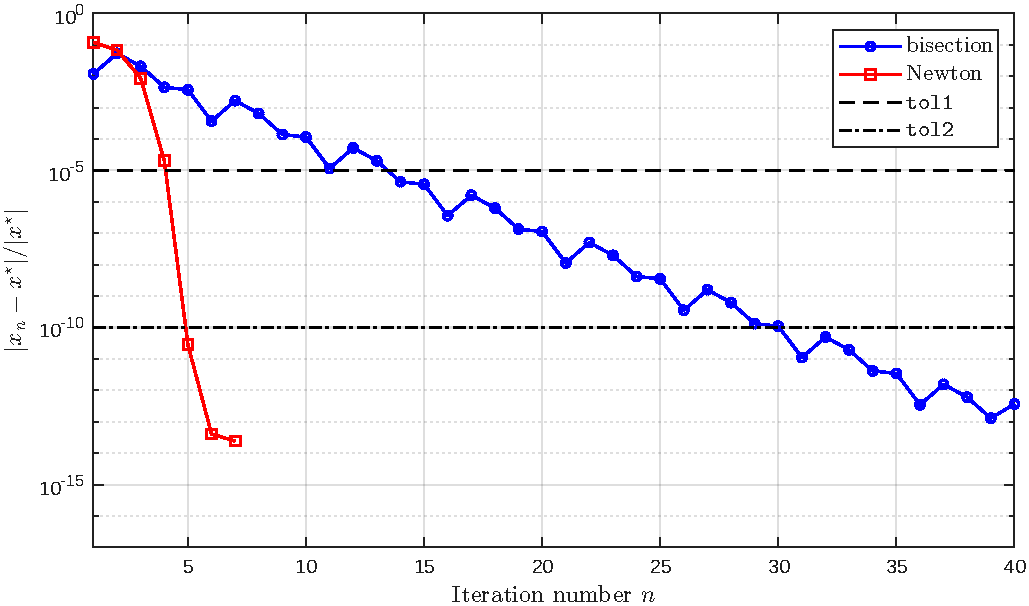
\includegraphics[width=0.78\textwidth]{fig2_convergence.pdf}
\caption{Linear versus quadratic convergence for the root near $x = 0.8436$.
Relative error against iteration number for bisection and for Newton started
from a comparable offset, with both tolerances marked. The bisection error
descends raggedly, since \eqref{eq:biserr} bounds it by a $2^{-n}$ envelope
without forcing a decrease at every step, but on average follows $0.30$ digits
per step. Newton reaches $\sim\!10^{-14}$ by $n = 6$, where it levels off at
the accuracy of the reference value rather than of the method.}
\label{fig:conv}
\end{figure}

\subsection{Problem 2}

Starting from $\mathbf{x}^{(0)} = (-1.00,\, 0.75,\, 1.50)$ with
$\texttt{tol} = 10^{-12}$, \texttt{newtond} converged in nine iterations to
%
\begin{equation}
(x, y, z) = (-0.577705133337,\; 0.447447204972,\; 1.084412371725) ,
\label{eq:root3d}
\end{equation}
%
with residual $\|\mathbf{f}\| = 2.5 \times 10^{-16}$. The relative update at
each step was
%
\begin{center}
\begin{tabular}{cl@{\qquad\qquad}cl}
\toprule
$n$ & $\|\boldsymbol{\delta}_n\|/\|\mathbf{x}_{n+1}\|$ &
$n$ & $\|\boldsymbol{\delta}_n\|/\|\mathbf{x}_{n+1}\|$ \\
\midrule
1 & $2.042 \times 10^{-1}$ & 6 & $5.686 \times 10^{-3}$  \\
2 & $1.345 \times 10^{-1}$ & 7 & $4.265 \times 10^{-4}$  \\
3 & $4.913 \times 10^{-2}$ & 8 & $7.024 \times 10^{-7}$  \\
4 & $1.935 \times 10^{-1}$ & 9 & $4.010 \times 10^{-13}$ \\
5 & $9.521 \times 10^{-2}$ &   &                         \\
\bottomrule
\end{tabular}
\end{center}
%
From $n = 6$ onward the exponent roughly doubles at each step, the signature of
quadratic convergence.

%=======================================================================
\section{Discussion and conclusions}
\label{sec:discussion}
%=======================================================================

Both of my routines performed as intended. In Problem 1 bisection reliably
delivered an estimate inside Newton's basin of convergence, after which Newton
reached \texttt{tol2} in a few steps, against the roughly twenty-three further
halvings bisection would have needed.

The residuals in Table~\ref{tab:roots} grow by seven orders of magnitude from
$k = 1$ to $k = 10$, but comparison with the exact roots shows the roots
themselves remain accurate. The growth comes from evaluating \eqref{eq:poly}
near $x = 2$, where terms of size $512 \times 2^{10} \approx 5\times10^5$ must
cancel to something of order unity. This leaves a round-off floor of about
$10^{-16} \times 5\times10^5 \approx 10^{-10}$ on the computed $f$, which is
where the largest residuals sit. It also limits roots 8--10 to a relative accuracy of a few $\times 10^{-12}$, whatever the value of \texttt{tol2}. Writing $f$ in the Chebyshev basis would avoid
this.

In Problem 2 the relative update grows between $n = 3$ and $n = 4$ before
recovering, so the given starting point is close enough for convergence but
not for the quadratic rate to hold from the start. Nothing in several
dimensions guards against this the way bisection does in Problem 1; damping the
step until the residual decreases would.

The main problem I had was interpreting the large residuals near $x = 2$ in
Table~\ref{tab:roots}. Until I noticed that $f(x) = T_{10}(x-1)$, I could not
tell whether they meant the roots there were inaccurate or were only round-off
in evaluating $f$. Problem 2 has no exact solution to compare against, so I
rely instead on the observed quadratic convergence and the machine-precision
residual as evidence that \texttt{newtond} found a genuine root.

\end{document}
